
Mean closeness cenrtality $\mathcal{C}$, as presented in \cite{newman2018networks}, is defined as follows:
\begin{align*}
 \mathcal{C} &= \dfrac{1}{N}\sum_{i=1}^N\mathcal{C}_i & \mathcal{C}_i &= \dfrac{1}{N-1}\sum_{\substack{j=1\\j\neq i}}^N \dfrac{1}{d_{ij}}& d_{ij} &=|P|
\end{align*}
Where $N$ is the number of nodes, $\mathcal{C}_i$ is the closeness centrality of vertex $i$, $d_{ij}$ is the geodesic distance between vertices $i$ and $j$, also as defined by \cite{newman2018networks}, and $P$ is the shortest path connecting edges $i$ and $j$ in the graph defined as a sequence (then $|P|$ is the length of said path).
\subsection{Description of the models}
\paragraph{Erdös-Rény model}
The Erdös-Rény model, also called binomial model, generates a random graph with a binomial process by flipping a coin and choosing whether an edge should be included or not. The used model is a slight variation of this one, because of instead of choosing the probability of an edge to be included or not, so the number of edges would follow a binomial distribution with expected value $\mathbb{E}[E] = p |E|$, the number of edges is fixed.
\paragraph{Switching model}
The switching model is a generator of random graphs given a degree sequence. This model has an interesting property to our experiments, because it preserve degrees although uniform sampling is not warranted.
\begin{algorithm}[!htb]
\caption{Switching mdodel}\label{algo:switching-model}
\begin{algorithmic}[line numbering]
\Require $G = (V,E), Q \in \mathbb{N}$
\For{$|E|\cdot Q$ times}
    \State $(u,v) \gets$ Choose u.a.r from $E$
    \State $(s,t) \gets$ Choose u.a.r from $E$
    \If{flip coin gets heads}
        \State Swap edges to $(u,t)$ and $(s,v)$
    \Else
        \State Swap edges to $(u,s)$ and $(v,t)$
    \EndIf
    \If{swap generates self-loops or parallel edges}
        \State Undo swap
    \EndIf
\EndFor
\end{algorithmic}
\end{algorithm}

The generation of graphs given a degree sequence yields multiple challenges adressed by some pieces in the literature \cite{blitzstein2011sequential, coolen2009constrained, milo2003uniform}. Our model deals with some of them, but to do so it lacks correctness in other areas. We believe this trade off is beneficial since the flawed properties of our implementation can be bounded. Some heuristics in our code are worth highlighting, referring to the Switching model:
\begin{itemize}
    \item Unbiased edge-picking. \\
    Asides from selecting a pair of edges to switch, we also check for possible switching randomly. Checking is referred not to the identification of failure switchings - those invalid because they don't preserve the degree sequence, but valid otherwise - but to the identification of switchings that pick the same edge to switch. Notice that since the graph is undirected, random selection of edges can yield a selected pair of edges $uv$,$vu$, where both $u,v\in V$ that are, in fact, the same edge. If this is not done, there is a bias because in our representation an edge is a pair of numbers in which the first one is smaller than the second. This bias causes that edges between nodes with smaller id or with high id are less probable.

    \item Guarantee of degree sequence preservation and impact on closeness centrality.\\
    The described implementation of the Switching model is flawed in the sense that it does not guarantee that no cycles are created. This can yield the generation of non-tree graphs, that although can otherwise show properties similar to those of SDN, fail to be acyclic as SDN are. This has a direct impact on the simulated closeness centrality. More detailed reasoning of this argument can be found in Appendix \ref{appendix:cc}.
\end{itemize}

\subsection{Implementation and execution}
The models have been implemented in C++ using the Boost Graph\footnote{See \url{https://www.boost.org/doc/libs/1_82_0/libs/graph/doc/index.html}} library \cite{siek2001boost}. We choose this library because it already implements some useful algorithms that we needed and also provides some representations for the graph. We used a adjacency list to represent the graph because the density is of edges (check table \ref{tab:1}) is low and this representation is really good for sparse graphs. In the switching model, we didn't used this representation because it does not allow to random access to the edges which is a frequent operation needed to this model. Therefore, we opted to use a \verb|std::vector| of pairs of integers to represent the edges and a \verb|std::set| of pairs in order to speed up the edge existence queries. 

Compilation flags include those recommended by the Boost library. Moreover, the repetitions of the trials for estimating the $p$-value has been parallelized using OpenMP allowing us to reduce the execution time of our experiments.

The experiments have been run with $Q = 1 +\log E$ for the switching model and the number of repetitions $T=100$ for all languages. Instead of computing bounds of the closeness centrality or its exact form, we opted to do a Montecarlo approximation with the 10\% of the nodes.

\subsection{Validation of the approximation of the closeness centrality \label{sub:validation}}
We chose to do an approximation of the closeness centrality by choosing a subset of the vertices and computing the closeness centrality between them. We decided that using the 10\% of the nodes to do this approximation was a reasonable amount in the trade-off between computational cost and approximation to the exact value.

In order to validate that our assumption was correct, we designed an experiment in which we run the method 100 times for the Catalan SDN, a binomial graph with the same number of vertices and edges as the Catalan SDN and applying the switching model $E \log E$ times to the Catalan SDN. Figure \ref{fig:validation} shows the results of the experiment in comparison with the exact computation of the metric. We observed that the approximations obtained are pretty close to the exact value, mainly for the binomial graph. The amount of error produced by this method can be observed in the third decimal and is evenly distributed above and below the real value, which allows us to conclude that the approximation is good enough to be used instead of the exact value.

\begin{figure}[!htb]
    \centering
    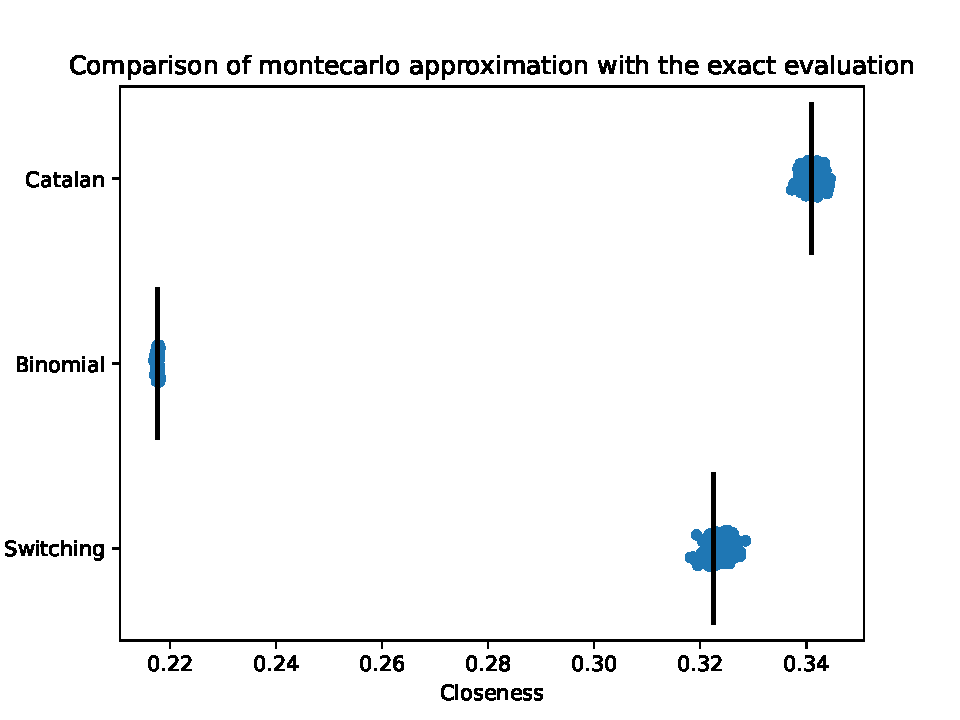
\includegraphics[width=0.75\textwidth]{figures/closeness_validation.pdf}
    \caption{Difference between the approximation and the exact value}
    \label{fig:validation}
\end{figure}